% THIS IS SIGPROC-SP.TEX - VERSION 3.1
% WORKS WITH V3.2SP OF ACM_PROC_ARTICLE-SP.CLS
% APRIL 2009
%
% It is an example file showing how to use the 'acm_proc_article-sp.cls' V3.2SP
% LaTeX2e document class file for Conference Proceedings submissions.
% ----------------------------------------------------------------------------------------------------------------
% This .tex file (and associated .cls V3.2SP) *DOES NOT* produce:
%       1) The Permission Statement
%       2) The Conference (location) Info information
%       3) The Copyright Line with ACM data
%       4) Page numbering
% ---------------------------------------------------------------------------------------------------------------
% It is an example which *does* use the .bib file (from which the .bbl file
% is produced).
% REMEMBER HOWEVER: After having produced the .bbl file,
% and prior to final submission,
% you need to 'insert'  your .bbl file into your source .tex file so as to provide
% ONE 'self-contained' source file.
%
% Questions regarding SIGS should be sent to
% Adrienne Griscti ---> griscti@acm.org
%
% Questions/suggestions regarding the guidelines, .tex and .cls files, etc. to
% Gerald Murray ---> murray@hq.acm.org
%
% For tracking purposes - this is V3.1SP - APRIL 2009

\documentclass{acm_proc_article-sp}

\begin{document}

\title{USB in a Microkernelenvironment}
\subtitle{[Extended Abstract]}
%
% You need the command \numberofauthors to handle the 'placement
% and alignment' of the authors beneath the title.
%
% For aesthetic reasons, we recommend 'three authors at a time'
% i.e. three 'name/affiliation blocks' be placed beneath the title.
%
% NOTE: You are NOT restricted in how many 'rows' of
% "name/affiliations" may appear. We just ask that you restrict
% the number of 'columns' to three.
%
% Because of the available 'opening page real-estate'
% we ask you to refrain from putting more than six authors
% (two rows with three columns) beneath the article title.
% More than six makes the first-page appear very cluttered indeed.
%
% Use the \alignauthor commands to handle the names
% and affiliations for an 'aesthetic maximum' of six authors.
% Add names, affiliations, addresses for
% the seventh etc. author(s) as the argument for the
% \additionalauthors command.
% These 'additional authors' will be output/set for you
% without further effort on your part as the last section in
% the body of your article BEFORE References or any Appendices.

\numberofauthors{2} %  in this sample file, there are a *total*
% of EIGHT authors. SIX appear on the 'first-page' (for formatting
% reasons) and the remaining two appear in the \additionalauthors section.
%
\author{
% You can go ahead and credit any number of authors here,
% e.g. one 'row of three' or two rows (consisting of one row of three
% and a second row of one, two or three).
%
% The command \alignauthor (no curly braces needed) should
% precede each author name, affiliation/snail-mail address and
% e-mail address. Additionally, tag each line of
% affiliation/address with \affaddr, and tag the
% e-mail address with \email.
%
% 1st. author
\alignauthor
Daniel Mierswa\\
       \affaddr{RheinMain University of Applied Sciences}\\
       \affaddr{Erlenweg 22}\\
       \affaddr{Taunusstein, Germany}\\
       \email{impulze@impulze.org}
% 2nd. author
\alignauthor
Daniel Tkocz\\
       \affaddr{RheinMain University of Applied Sciences}\\
       \affaddr{Schiffergasse 15}\\
       \affaddr{Wiesbaden, Germany}\\
       \email{daniel.tkocz42@gmail.com}
}
% There's nothing stopping you putting the seventh, eighth, etc.
% author on the opening page (as the 'third row') but we ask,
% for aesthetic reasons that you place these 'additional authors'
% in the \additional authors block, viz.
%\additionalauthors{Additional authors: John Smith (The Th{\o}rv{\"a}ld Group,
%email: {\texttt{jsmith@affiliation.org}}) and Julius P.~Kumquat
%(The Kumquat Consortium, email: {\texttt{jpkumquat@consortium.net}}).}
%\date{30 July 1999}
% Just remember to make sure that the TOTAL number of authors
% is the number that will appear on the first page PLUS the
% number that will appear in the \additionalauthors section.

\maketitle
\begin{abstract}
This paper provides an introduction in using USB in a microkernel.
This paper also contains a small introduction in USB and microkernels for better understanding. Problems that might occur are described and solutions are presented.
%This paper provides a sample of a \LaTeX\ document which conforms to
%the formatting guidelines for ACM SIG Proceedings.
%It complements the document \textit{Author's Guide to Preparing
%ACM SIG Proceedings Using \LaTeX$2_\epsilon$\ and Bib\TeX}. This
%source file has been written with the intention of being
%compiled under \LaTeX$2_\epsilon$\ and BibTeX.

%The developers have tried to include every imaginable sort
%of ``bells and whistles", such as a subtitle, footnotes on
%title, subtitle and authors, as well as in the text, and
%every optional component (e.g. Acknowledgments, Additional
%Authors, Appendices), not to mention examples of
%equations, theorems, tables and figures.

%To make best use of this sample document, run it through \LaTeX\
%and BibTeX, and compare this source code with the printed
%output produced by the dvi file.
\end{abstract}

% A category with the (minimum) three required fields
%\category{H.4}{Information Systems Applications}{Miscellaneous}
%A category including the fourth, optional field follows...
%\category{D.2.8}{Software Engineering}{Metrics}[complexity measures, performance measures]

%\terms{Theory}

\keywords{USB, Microkernel, seL4} % NOT required for Proceedings

\section{Introduction}
In the 90's microkernels became more relevant and were developed more than before.
1996 USB was introduced.
This paper is about bringing those two technologies together.\\
Section \ref{sec:usb} is a small and general introduction in USB.
Section \ref{sec:microkernel} describes the structure of a microkernel.
Section \ref{sec:both} describes problems that may occur in a microkernelenvironment using USB and offers solutions.
\section{USB}
\label{sec:usb}
\begin{figure}
\centering

\includegraphics[width=0.2\textwidth]{usblogo.jpg}
\label{fig:usblogo}
\caption{USB 3.0 logo}
\end{figure}
USB (Universal Serial Bus) is a serial bus.
With USB it is possible to connect a lot of different types of devices with a host.
Today the most common USB-devices are keyboards and mice. But also external storage, mobilephones and gadgets like a small rocketlauncher can be connected to a host by USB. USB supports hotplugging of USB-devices. That means connecting and disconnecting a USB-device to/from a running host and detecting the USB-device.
\subsection{Hardware}
There is a large amount of different USB-connectors (Type A, Type B, Mini A, Mini AB, Mini B, Micro AB, Micro B, Type C). They vary in size, profile, durability, compability and usability.
The used pins used in USB 1.x/2.0 in each of the connectors are nearly the same.

\begin{table}
\centering
\caption{USB 1.x/2.0 standard pinout}
\begin{tabular}{|l|l|l|l|} \hline
Pin & Name & Wire color & Description\\ \hline
1 & $V_{BUS}$ & Red (or orange) & + 5 V\\ \hline
2 & D- & White (or gold) & Data-\\ \hline
3 & D+ & Green & Data+\\ \hline
4 & GND & Black (or blue) & Ground\\ \hline
\end{tabular}
\end{table}

\begin{table}
\centering
\caption{USB 1.x/2.0 mini/micro pinout}
\begin{tabular}{|l|l|l|l|} \hline
Pin & Name & Wire color & Description\\ \hline
1 & $V_{BUS}$ & Red & + 5 V\\ \hline
2 & D- & White & Data-\\ \hline
3 & D+ & Green & Data+\\ \hline
4 & ID &  & Detect which connector is connected\\ \hline
5 & GND & Black & Ground\\ \hline
\end{tabular}
\end{table}

Only USB 3.x varies a lot. But some USB 3.0 connectors are backwardcompatible.
$V_{BUS}$ and GND supply the connected device with power varing from specification from 0.5 A to 3 A at 5 V in general. The wires in a USB-cable are twisted to reduce noise. The communication in USB 1.x/2.0 is half-duplex, USB 3.x is full-duplex.
Depending on USB-version the datarate is 1.5 Mbit/s up to 10 Gbit/s. USB 2.0 has a datarate of 480 Mbit/s.

\subsection{Software} %http://www.beyondlogic.org/usbnutshell/usb1.shtml
\subsubsection{Device Descriptor} %http://www.usb.org/developers
The device descriptor specify a couple of informations about a device.
All informations can be printed on the console of a linuxsystem by entering \emph{lsusb -v} in the console. The devicedescriptor is only one descriptor from a small group. There exists the configurationdescriptor -- which describes how much power the device needs, which powermode is used (sleep, selfpowered, etc.), etc. -- , the endpointdescriptor -- described later -- , the interfaceendpoint -- which bundles a group of endpointdesciptors -- and stringdescriptors -- which contain a single string instead of hex-numbers.
\paragraph{USB Version}
The devicedescriptor specify the used USB-version. By manipulating this field in the devicedescriptor, a USB 2.0 device can connect to a host as USB 1.1-device.
\paragraph{Device Class}
To specify the functionality of a device class codes are used. They are communicated to the host to determine if the device is supported and if so decide which driver should be used for it. For example a device identifiying itself with the classcode $0E_h$ should be treated as a webcam providing a videosignal. In compare to that a device sending $03_h$ should be treated as a human-interface-device (keyboard, mouse, etc.).
If no devicespecific driver exists, in general a generic driver will try to control the device. If the manufacturer thinks none of the deviceclasses matches his needs, the manufacturer can decide to use a vendor specific class: $FF_h$. This might be a good idea for a USB-rocketlauncher.
\paragraph{Device SubClass}
The subclass specifies more detailed than the device class what the device is.
\paragraph{Device Protocol}
The protocol field defines a protocol which should be used to communicate with it.
\paragraph{IDs \& Numbers}
The devicedescriptor contains a vendor-id to identify the manufacturer of a device.
To identify the product of a manufacturer, a product-id is used. To specify the hardwareconfiguration furthermore a device-release-number and a serial number can be specified.

\subsubsection{Endpoints}
Endpoints are used for communication. Each communication is directed to a specific endpoint. A device/host might have multiple endpoints for different purposes. There are four different types of endpoints. The integrity of a transfer is secured by a CRC-sum for each Endpoint. To end a transfer, each mesage needs to be acknowleged except those from interruptendpoints. Endpoints are configured in an endpointdescriptor. In general the communication has three parts:
\begin{itemize}
\item Token Packet
\item Data Packet
\item Handshake Packet
\end{itemize}
Tokenpackets specify the direction of the communication relative to the host. IN means, the host receives data from the device, OUT means the host sends data to the device.\\
Datapackets contains the data or if the passive side of the communication is not ready, it can send STALL or do not respond within a few milliseconds.
\begin{figure}
\centering
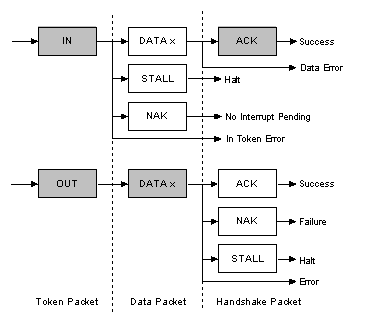
\includegraphics[width=0.4\textwidth]{interrupttransfer.png}
\label{fig:interrupttransfer}
\caption{Protocol of an interrupttransfer}
\end{figure}
\paragraph{Control Endpoint}
Controlendpoints are used for controltransfers. With them the device is configured. Every device has a controlendpoint (endpoint zero).
\paragraph{Bulk Endpoint}
Bulkendpoints are used for bulktransfers. Bulktransfers are non timecritically, large datatransfers for example a read-/writeoperation on a external storagedevice.
\paragraph{Isochronus Endpoint}
Isochronusendpoints are used for isochronustransfers. Isochronustransfers are used if a specific datarate is required.
\paragraph{Interrupt Endpoint}
Interruptendpoints are used for interrupttransfers. Other than expected in USB 2.0 and lower this endpoint does not really work with interrupts. Interrupttransfers are polled each x milliseconds. They are often used for human-interface-devices.
\subsection{Packets}
For the complete communication packets are used. Each message send from an endpoint and received from an endpoint is based on a simple USB-packet. The packetoverhead is only a few bytes depending on used USB-version. Depending on packettype the packet may contain the following data.
\paragraph{Sync}
All packets start with a sync field. The field is used to synchronise the timing of transmitter and receiver.
\paragraph{PID}
To specify the content of a packet each sync field of a packet is followed by a PID-field. It contains a 4 bit information about the content. To ensure integrity the PID field contains twice the information to detect biterrors.
\paragraph{ADDR}
The ADDR field specifies a divice to communicate with.
\paragraph{ENDP}
The ENDP field specifies an endpoint which should receive the packet. Other Endpoints will not notice the packet at all.
\paragraph{Data}
The datafield contains up to 1 KB custom data.
\paragraph{CRC}
The CRC field contains a CRC sum \emph{only} of the datafield to ensure integrity of the data.
\paragraph{EOP}
The EOP-field indicates the end of the package and is everytime the last in field in each package.
\section{Microkernel}
\label{sec:microkernel}
A microkernel ($\mu$-kernel) as opposed to a monolothic kernel has fewer code running in
supervisor mode (kernel mode).
\begin{figure}
\centering
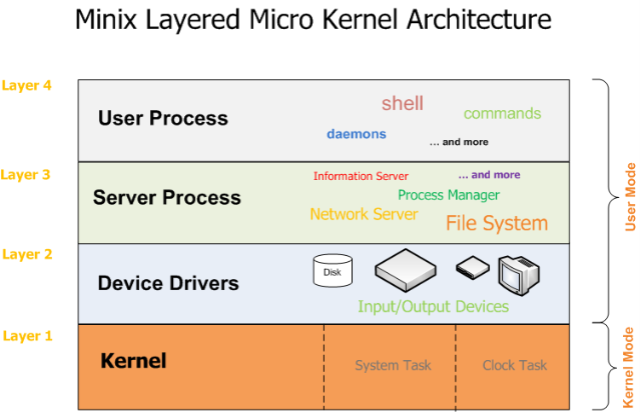
\includegraphics[width=0.4\textwidth]{minixinternalstructure.png}
\label{fig:minixmicarch}
\caption{The microkernel architecture as provided by Minix [minixref]}
\end{figure}
The architecture in of microkernel based operating systems separates basic
hardware functionality from other portions (as seen in Figure \ref{fig:minixmicarch}).
The modularization, if stricly executed, makes it easier for developers to support new
platforms since they only have to port the machine-dependent code for basic hardware functionality.
[black92microkernel]
The code for system specific functionality (services) runs in user mode and as such
is not capable of interfering directly with hardware.
This demonstrates a challenge for driver developers and requires a well-defined kernel API.
Due to the separation and indirection it is believed that microkernels cannot perform as well as
monolithic kernels.
However, most of the performance issues of first generation microkernels were based on poor design
and faulty implementations [p237-liedtke].
Furthermore, device drivers implemented as services on microkernel operating systems can achieve
almost the same performance as monolithic drivers [uldd].

\subsection{Generations}
The idea of a microkernel was introduced in the late 1980s, however at this point Unix [refunix]
was already widely used and adopted.
The concepts of Unix worked good enough around that time and BSD [refbsd] adoption of Unix started
the era of big kernels through adding filesystems and a complete TCP/IP stack. [wiki]
The amount of code in kernels grew fast and with each new code fragment the possibilities of
freezing a system from within a faulty driver implementation increased.
Supporters of microkernel based operating systems argued that user-level implemented TCP/IP drivers
would simply restart the driver and leave the other OS functionality undamaged.
The Mach [refmach] microkernel was developed as a replacement to the mentioned BSD Unix.
It was developed from 1985 to the mid 90s at Carnegie Mellon University and is considered to be
the system that defines the first generation of microkernels.

Mach's external pager [p70liedtke] which manages physical and virtual memory in a way that allows
user-level code to map files and databases into their address space without using the filesystem
driver.
It also llowed the usage of multiple systems simultaenously [p70liedtke].
Another early idea was to implement Interrupt handling via Inter Process Communication (IPC).
IPC is the core component of any microkernel based operating system.
User-level servers can send/receive messages to/from the kernel or other user-level servers
through the kernel.
As one can see the implementation of the communication protocol is a bottleneck and optimization
is necessary to meet the requirements of todays applications.
Analysis of performance problems [p70liedtke] showed that user-kernel-mode switches, address-space
switches and memory penalties also contributed to a bad performance.

In the mid 90s development of new microkernels started.
They were written from scratch rather than evolving from the present monolithic kernels.
One of them was L4 [l4ref].
L4 has three abstraction layers: address spaces, threads and IPC.
Based on tests on a 486-DX5 machine the L4 microkernel RPC was twice as fast as a UNIX system call
and 20 times faster than first generation IPC [p70liedtke].
The address space concept removed another limitation of first generation microkernels.
Basically you were allowed to recursively construct address spaces outside the kernel.
Memory management concepts used in the L4 kernel interface were an extension of the external
pager mechanisms presented in Mach kernels.

\section{USB in Microkernels}
\label{sec:both}
Earlier we presented the basic architecture of USB and how communication works on the serial bus.
In the previous chapter we've seen that microkernels are capable of accessing shared resources
(e.g. a bus) through APIs.
The obvious simple approach to support USB in a microkernel based operating system would be to provide
a service for the interaction with the Host Controller (HC) and let USB device drivers use the HC service.
If another USB device driver uses the HC service the URB coming from this device driver would be
blocked or queued.
This approach would work in a simple 1-to-1 relation when an operating system would just interact
with one USB device.
In real world scenarios however we often face situations where one application (client) uses one or more
devices (interfacing with one or more device drivers), several applications use one or more devices or
devices communicating with each other (data transfer between mass-storage devices).
A simmple ''blocking'' approach does not suffice and another component has to be provided to create a working
environment for USB device drivers.
It has to
\begin{itemize}
\item create URBs based on certain scheduling parameters to avoid blocking
\item fragment data so devices can be polled during huge data transfers
\item prevent unauthorized bus access by other drivers
\end{itemize}
In this paper we try to present a separated USB service which will encapsulate this functionality.

\subsection{USB service}
We'll look at the Linux USB driver architecture to get an understanding of how to separate concerns
in the handling of the USB protocol and introduce terms we'll be using when describing the design
of the USB service.
\begin{figure}
\centering
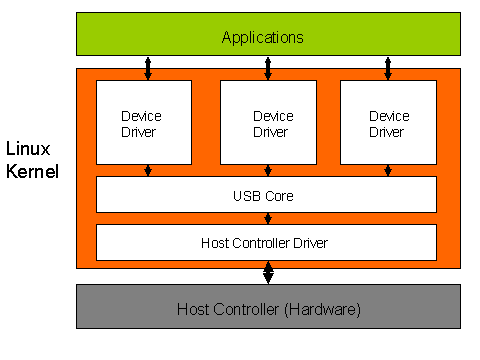
\includegraphics[width=0.4\textwidth]{usblinux.png}
\label{fig:usblinux}
\caption{Main components of the Linux USB driver}
\end{figure}
Figure \ref{fig:usblinux} shows how the operating system USB functionality can be split up into
major components.
The 3 components are:
\begin{itemize}
\item Driver for the Host Controller
\item USBCore support library
\item Drivers for USB devices
\end{itemize}
The USBCore library is used to abstract functionality of the Host Controller without knowing
the details of the platform like handling interrupts, memory access and configuration.
For the device drivers an interface is provided to manage memory and transfer data.
In addition it provides the USB Request Block (URB) for the specific implementation and ways
to communicate them.


\subsection{Difficulties}
\subsection{Solutionproposals}
\section{Conclusion}
\section{}
\section{Introduction}
The \textit{proceedings} are the records of a conference.
ACM seeks to give these conference by-products a uniform,
high-quality appearance.  To do this, ACM has some rigid
requirements for the format of the proceedings documents: there
is a specified format (balanced  double columns), a specified
set of fonts (Arial or Helvetica and Times Roman) in
certain specified sizes (for instance, 9 point for body copy),
a specified live area (18 $\times$ 23.5 cm [7" $\times$ 9.25"]) centered on
the page, specified size of margins (1.9 cm [0.75"]) top, (2.54 cm [1"]) bottom
and (1.9 cm [.75"]) left and right; specified column width
(8.45 cm [3.33"]) and gutter size (.83 cm [.33"]).

The good news is, with only a handful of manual
settings\footnote{Two of these, the {\texttt{\char'134 numberofauthors}}
and {\texttt{\char'134 alignauthor}} commands, you have
already used; another, {\texttt{\char'134 balancecolumns}}, will
be used in your very last run of \LaTeX\ to ensure
balanced column heights on the last page.}, the \LaTeX\ document
class file handles all of this for you.

The remainder of this document is concerned with showing, in
the context of an ``actual'' document, the \LaTeX\ commands
specifically available for denoting the structure of a
proceedings paper, rather than with giving rigorous descriptions
or explanations of such commands.

\section{The {\secit Body} of The Paper}
Typically, the body of a paper is organized
into a hierarchical structure, with numbered or unnumbered
headings for sections, subsections, sub-subsections, and even
smaller sections.  The command \texttt{{\char'134}section} that
precedes this paragraph is part of such a
hierarchy.\footnote{This is the second footnote.  It
starts a series of three footnotes that add nothing
informational, but just give an idea of how footnotes work
and look. It is a wordy one, just so you see
how a longish one plays out.} \LaTeX\ handles the numbering
and placement of these headings for you, when you use
the appropriate heading commands around the titles
of the headings.  If you want a sub-subsection or
smaller part to be unnumbered in your output, simply append an
asterisk to the command name.  Examples of both
numbered and unnumbered headings will appear throughout the
balance of this sample document.

Because the entire article is contained in
the \textbf{document} environment, you can indicate the
start of a new paragraph with a blank line in your
input file; that is why this sentence forms a separate paragraph.

\subsection{Type Changes and {\subsecit Special} Characters}
We have already seen several typeface changes in this sample.  You
can indicate italicized words or phrases in your text with
the command \texttt{{\char'134}textit}; emboldening with the
command \texttt{{\char'134}textbf}
and typewriter-style (for instance, for computer code) with
\texttt{{\char'134}texttt}.  But remember, you do not
have to indicate typestyle changes when such changes are
part of the \textit{structural} elements of your
article; for instance, the heading of this subsection will
be in a sans serif\footnote{A third footnote, here.
Let's make this a rather short one to
see how it looks.} typeface, but that is handled by the
document class file. Take care with the use
of\footnote{A fourth, and last, footnote.}
the curly braces in typeface changes; they mark
the beginning and end of
the text that is to be in the different typeface.

You can use whatever symbols, accented characters, or
non-English characters you need anywhere in your document;
you can find a complete list of what is
available in the \textit{\LaTeX\
User's Guide}\cite{Lamport:LaTeX}.

\subsection{Math Equations}
You may want to display math equations in three distinct styles:
inline, numbered or non-numbered display.  Each of
the three are discussed in the next sections.

\subsubsection{Inline (In-text) Equations}
A formula that appears in the running text is called an
inline or in-text formula.  It is produced by the
\textbf{math} environment, which can be
invoked with the usual \texttt{{\char'134}begin. . .{\char'134}end}
construction or with the short form \texttt{\$. . .\$}. You
can use any of the symbols and structures,
from $\alpha$ to $\omega$, available in
\LaTeX\cite{Lamport:LaTeX}; this section will simply show a
few examples of in-text equations in context. Notice how
this equation: \begin{math}\lim_{n\rightarrow \infty}x=0\end{math},
set here in in-line math style, looks slightly different when
set in display style.  (See next section).

\subsubsection{Display Equations}
A numbered display equation -- one set off by vertical space
from the text and centered horizontally -- is produced
by the \textbf{equation} environment. An unnumbered display
equation is produced by the \textbf{displaymath} environment.

Again, in either environment, you can use any of the symbols
and structures available in \LaTeX; this section will just
give a couple of examples of display equations in context.
First, consider the equation, shown as an inline equation above:
\begin{equation}\lim_{n\rightarrow \infty}x=0\end{equation}
Notice how it is formatted somewhat differently in
the \textbf{displaymath}
environment.  Now, we'll enter an unnumbered equation:
\begin{displaymath}\sum_{i=0}^{\infty} x + 1\end{displaymath}
and follow it with another numbered equation:
\begin{equation}\sum_{i=0}^{\infty}x_i=\int_{0}^{\pi+2} f\end{equation}
just to demonstrate \LaTeX's able handling of numbering.

\subsection{Citations}
Citations to articles \cite{bowman:reasoning, clark:pct, braams:babel, herlihy:methodology},
conference
proceedings \cite{clark:pct} or books \cite{salas:calculus, Lamport:LaTeX} listed
in the Bibliography section of your
article will occur throughout the text of your article.
You should use BibTeX to automatically produce this bibliography;
you simply need to insert one of several citation commands with
a key of the item cited in the proper location in
the \texttt{.tex} file \cite{Lamport:LaTeX}.
The key is a short reference you invent to uniquely
identify each work; in this sample document, the key is
the first author's surname and a
word from the title.  This identifying key is included
with each item in the \texttt{.bib} file for your article.

The details of the construction of the \texttt{.bib} file
are beyond the scope of this sample document, but more
information can be found in the \textit{Author's Guide},
and exhaustive details in the \textit{\LaTeX\ User's
Guide}\cite{Lamport:LaTeX}.

This article shows only the plainest form
of the citation command, using \texttt{{\char'134}cite}.
This is what is stipulated in the SIGS style specifications.
No other citation format is endorsed.

\subsection{Tables}
Because tables cannot be split across pages, the best
placement for them is typically the top of the page
nearest their initial cite.  To
ensure this proper ``floating'' placement of tables, use the
environment \textbf{table} to enclose the table's contents and
the table caption.  The contents of the table itself must go
in the \textbf{tabular} environment, to
be aligned properly in rows and columns, with the desired
horizontal and vertical rules.  Again, detailed instructions
on \textbf{tabular} material
is found in the \textit{\LaTeX\ User's Guide}.

Immediately following this sentence is the point at which
Table 1 is included in the input file; compare the
placement of the table here with the table in the printed
dvi output of this document.

\begin{table}
\centering
\caption{Frequency of Special Characters}
\begin{tabular}{|c|c|l|} \hline
Non-English or Math&Frequency&Comments\\ \hline
\O & 1 in 1,000& For Swedish names\\ \hline
$\pi$ & 1 in 5& Common in math\\ \hline
\$ & 4 in 5 & Used in business\\ \hline
$\Psi^2_1$ & 1 in 40,000& Unexplained usage\\
\hline\end{tabular}
\end{table}

To set a wider table, which takes up the whole width of
the page's live area, use the environment
\textbf{table*} to enclose the table's contents and
the table caption.  As with a single-column table, this wide
table will ``float" to a location deemed more desirable.
Immediately following this sentence is the point at which
Table 2 is included in the input file; again, it is
instructive to compare the placement of the
table here with the table in the printed dvi
output of this document.


\begin{table*}
\centering
\caption{Some Typical Commands}
\begin{tabular}{|c|c|l|} \hline
Command&A Number&Comments\\ \hline
\texttt{{\char'134}alignauthor} & 100& Author alignment\\ \hline
\texttt{{\char'134}numberofauthors}& 200& Author enumeration\\ \hline
\texttt{{\char'134}table}& 300 & For tables\\ \hline
\texttt{{\char'134}table*}& 400& For wider tables\\ \hline\end{tabular}
\end{table*}
% end the environment with {table*}, NOTE not {table}!

\subsection{Figures}
Like tables, figures cannot be split across pages; the
best placement for them
is typically the top or the bottom of the page nearest
their initial cite.  To ensure this proper ``floating'' placement
of figures, use the environment
\textbf{figure} to enclose the figure and its caption.

This sample document contains examples of \textbf{.eps}
and \textbf{.ps} files to be displayable with \LaTeX.  More
details on each of these is found in the \textit{Author's Guide}.

\begin{figure}
\centering
%\epsfig{file=fly.eps}
\caption{A sample black and white graphic (.eps format).}
\end{figure}

\begin{figure}
\centering
%\epsfig{file=fly.eps, height=1in, width=1in}
\caption{A sample black and white graphic (.eps format)
that has been resized with the \texttt{epsfig} command.}
\end{figure}


As was the case with tables, you may want a figure
that spans two columns.  To do this, and still to
ensure proper ``floating'' placement of tables, use the environment
\textbf{figure*} to enclose the figure and its caption.

Note that either {\textbf{.ps}} or {\textbf{.eps}} formats are
used; use
the \texttt{{\char'134}epsfig} or \texttt{{\char'134}psfig}
commands as appropriate for the different file types.

\subsection{Theorem-like Constructs}
Other common constructs that may occur in your article are
the forms for logical constructs like theorems, axioms,
corollaries and proofs.  There are
two forms, one produced by the
command \texttt{{\char'134}newtheorem} and the
other by the command \texttt{{\char'134}newdef}; perhaps
the clearest and easiest way to distinguish them is
to compare the two in the output of this sample document:

This uses the \textbf{theorem} environment, created by
the\linebreak\texttt{{\char'134}newtheorem} command:
\newtheorem{theorem}{Theorem}
\begin{theorem}
Let $f$ be continuous on $[a,b]$.  If $G$ is
an antiderivative for $f$ on $[a,b]$, then
\begin{displaymath}\int^b_af(t)dt = G(b) - G(a).\end{displaymath}
\end{theorem}

The other uses the \textbf{definition} environment, created
by the \texttt{{\char'134}newdef} command:
\newdef{definition}{Definition}
\begin{definition}
If $z$ is irrational, then by $e^z$ we mean the
unique number which has
logarithm $z$: \begin{displaymath}{\log e^z = z}\end{displaymath}
\end{definition}

\begin{figure}
\centering
%\psfig{file=rosette.ps, height=1in, width=1in,}
\caption{A sample black and white graphic (.ps format) that has
been resized with the \texttt{psfig} command.}
\end{figure}

Two lists of constructs that use one of these
forms is given in the
\textit{Author's  Guidelines}.

\begin{figure*}
\centering
%\epsfig{file=flies.eps}
\caption{A sample black and white graphic (.eps format)
that needs to span two columns of text.}
\end{figure*}
and don't forget to end the environment with
{figure*}, not {figure}!
 
There is one other similar construct environment, which is
already set up
for you; i.e. you must \textit{not} use
a \texttt{{\char'134}newdef} command to
create it: the \textbf{proof} environment.  Here
is a example of its use:
\begin{proof}
Suppose on the contrary there exists a real number $L$ such that
\begin{displaymath}
\lim_{x\rightarrow\infty} \frac{f(x)}{g(x)} = L.
\end{displaymath}
Then
\begin{displaymath}
l=\lim_{x\rightarrow c} f(x)
= \lim_{x\rightarrow c}
\left[ g{x} \cdot \frac{f(x)}{g(x)} \right ]
= \lim_{x\rightarrow c} g(x) \cdot \lim_{x\rightarrow c}
\frac{f(x)}{g(x)} = 0\cdot L = 0,
\end{displaymath}
which contradicts our assumption that $l\neq 0$.
\end{proof}

Complete rules about using these environments and using the
two different creation commands are in the
\textit{Author's Guide}; please consult it for more
detailed instructions.  If you need to use another construct,
not listed therein, which you want to have the same
formatting as the Theorem
or the Definition\cite{salas:calculus} shown above,
use the \texttt{{\char'134}newtheorem} or the
\texttt{{\char'134}newdef} command,
respectively, to create it.

\subsection*{A {\secit Caveat} for the \TeX\ Expert}
Because you have just been given permission to
use the \texttt{{\char'134}newdef} command to create a
new form, you might think you can
use \TeX's \texttt{{\char'134}def} to create a
new command: \textit{Please refrain from doing this!}
Remember that your \LaTeX\ source code is primarily intended
to create camera-ready copy, but may be converted
to other forms -- e.g. HTML. If you inadvertently omit
some or all of the \texttt{{\char'134}def}s recompilation will
be, to say the least, problematic.

\section{Conclusions}
This paragraph will end the body of this sample document.
Remember that you might still have Acknowledgments or
Appendices; brief samples of these
follow.  There is still the Bibliography to deal with; and
we will make a disclaimer about that here: with the exception
of the reference to the \LaTeX\ book, the citations in
this paper are to articles which have nothing to
do with the present subject and are used as
examples only.
%\end{document}  % This is where a 'short' article might terminate

%ACKNOWLEDGMENTS are optional
\section{Acknowledgments}
This section is optional; it is a location for you
to acknowledge grants, funding, editing assistance and
what have you.  In the present case, for example, the
authors would like to thank Gerald Murray of ACM for
his help in codifying this \textit{Author's Guide}
and the \textbf{.cls} and \textbf{.tex} files that it describes.

%
% The following two commands are all you need in the
% initial runs of your .tex file to
% produce the bibliography for the citations in your paper.
\bibliographystyle{abbrv}
\bibliography{sigproc}  % sigproc.bib is the name of the Bibliography in this case
% You must have a proper ".bib" file
%  and remember to run:
% latex bibtex latex latex
% to resolve all references
%
% ACM needs 'a single self-contained file'!
%
%APPENDICES are optional
%\balancecolumns
\appendix
%Appendix A
\section{Headings in Appendices}
The rules about hierarchical headings discussed above for
the body of the article are different in the appendices.
In the \textbf{appendix} environment, the command
\textbf{section} is used to
indicate the start of each Appendix, with alphabetic order
designation (i.e. the first is A, the second B, etc.) and
a title (if you include one).  So, if you need
hierarchical structure
\textit{within} an Appendix, start with \textbf{subsection} as the
highest level. Here is an outline of the body of this
document in Appendix-appropriate form:
\subsection{Introduction}
\subsection{The Body of the Paper}
\subsubsection{Type Changes and  Special Characters}
\subsubsection{Math Equations}
\paragraph{Inline (In-text) Equations}
\paragraph{Display Equations}
\subsubsection{Citations}
\subsubsection{Tables}
\subsubsection{Figures}
\subsubsection{Theorem-like Constructs}
\subsubsection*{A Caveat for the \TeX\ Expert}
\subsection{Conclusions}
\subsection{Acknowledgments}
\subsection{Additional Authors}
This section is inserted by \LaTeX; you do not insert it.
You just add the names and information in the
\texttt{{\char'134}additionalauthors} command at the start
of the document.
\subsection{References}
Generated by bibtex from your ~.bib file.  Run latex,
then bibtex, then latex twice (to resolve references)
to create the ~.bbl file.  Insert that ~.bbl file into
the .tex source file and comment out
the command \texttt{{\char'134}thebibliography}.
% This next section command marks the start of
% Appendix B, and does not continue the present hierarchy
\section{More Help for the Hardy}
The acm\_proc\_article-sp document class file itself is chock-full of succinct
and helpful comments.  If you consider yourself a moderately
experienced to expert user of \LaTeX, you may find reading
it useful but please remember not to change it.
\balancecolumns
% That's all folks!
\end{document}
